\documentclass[../main.tex]{subfiles}


\begin{document}


\tikzset{every picture/.style={line width=0.75pt}} %set default line width to 0.75pt        

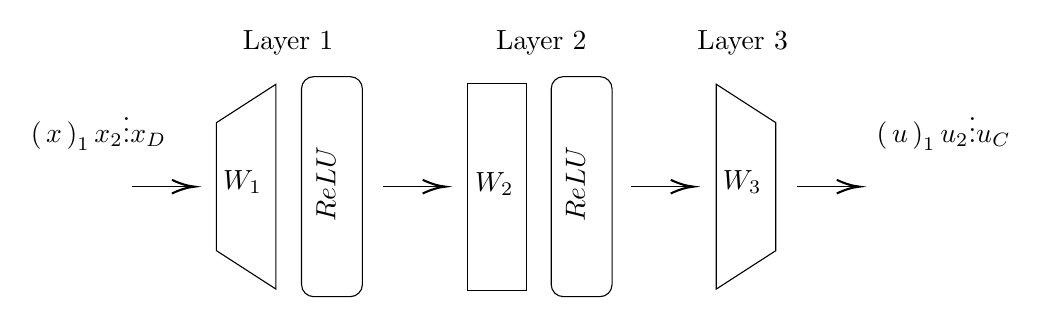
\begin{tikzpicture}[x=0.75pt,y=0.75pt,yscale=-1,xscale=1]
%uncomment if require: \path (0,200); %set diagram left start at 0, and has height of 200

%Flowchart: Manual Operation [id:dp9126982954216896] 
\draw   (150.17,69.5) -- (178.83,51) -- (178.83,149.67) -- (150.17,131.17) -- cycle ;

%Straight Lines [id:da20688044961383312] 
\draw    (109.67,100.33) -- (137.67,100.33) ;
\draw [shift={(139.67,100.33)}, rotate = 180] [color={rgb, 255:red, 0; green, 0; blue, 0 }  ][line width=0.75]    (10.93,-3.29) .. controls (6.95,-1.4) and (3.31,-0.3) .. (0,0) .. controls (3.31,0.3) and (6.95,1.4) .. (10.93,3.29)   ;
%Rounded Rect [id:dp9737700870951371] 
\draw   (214.63,47.33) .. controls (217.87,47.33) and (220.5,49.96) .. (220.5,53.2) -- (220.5,147.47) .. controls (220.5,150.71) and (217.87,153.33) .. (214.63,153.33) -- (197.03,153.33) .. controls (193.79,153.33) and (191.17,150.71) .. (191.17,147.47) -- (191.17,53.2) .. controls (191.17,49.96) and (193.79,47.33) .. (197.03,47.33) -- cycle ;

%Shape: Rectangle [id:dp8599103849713333] 
\draw   (271.03,50.46) -- (299.5,50.46) -- (299.5,150.21) -- (271.03,150.21) -- cycle ;

%Rounded Rect [id:dp6266699612098101] 
\draw   (334.93,47.33) .. controls (338.17,47.33) and (340.8,49.96) .. (340.8,53.2) -- (340.8,147.47) .. controls (340.8,150.71) and (338.17,153.33) .. (334.93,153.33) -- (317.33,153.33) .. controls (314.09,153.33) and (311.47,150.71) .. (311.47,147.47) -- (311.47,53.2) .. controls (311.47,49.96) and (314.09,47.33) .. (317.33,47.33) -- cycle ;

%Straight Lines [id:da5605900304491034] 
\draw    (230.5,100.33) -- (258.5,100.33) ;
\draw [shift={(260.5,100.33)}, rotate = 180] [color={rgb, 255:red, 0; green, 0; blue, 0 }  ][line width=0.75]    (10.93,-3.29) .. controls (6.95,-1.4) and (3.31,-0.3) .. (0,0) .. controls (3.31,0.3) and (6.95,1.4) .. (10.93,3.29)   ;
%Straight Lines [id:da2864685222655661] 
\draw    (350,100.33) -- (378,100.33) ;
\draw [shift={(380,100.33)}, rotate = 180] [color={rgb, 255:red, 0; green, 0; blue, 0 }  ][line width=0.75]    (10.93,-3.29) .. controls (6.95,-1.4) and (3.31,-0.3) .. (0,0) .. controls (3.31,0.3) and (6.95,1.4) .. (10.93,3.29)   ;
%Flowchart: Manual Operation [id:dp8273257345355105] 
\draw   (419.67,131.17) -- (391,149.67) -- (391,51) -- (419.67,69.5) -- cycle ;

%Straight Lines [id:da3132194576411018] 
\draw    (430,100.33) -- (458,100.33) ;
\draw [shift={(460,100.33)}, rotate = 180] [color={rgb, 255:red, 0; green, 0; blue, 0 }  ][line width=0.75]    (10.93,-3.29) .. controls (6.95,-1.4) and (3.31,-0.3) .. (0,0) .. controls (3.31,0.3) and (6.95,1.4) .. (10.93,3.29)   ;

% Text Node
\draw (152.14,91.4) node [anchor=north west][inner sep=0.75pt]    {$W_{1}$};
% Text Node
\draw (59.5,57.73) node [anchor=north west][inner sep=0.75pt]    {$\begin{pmatrix}
x_{1}\\
x_{2}\\
\vdots \\
x_{D}
\end{pmatrix}$};
% Text Node
\draw (197.05,118.33) node [anchor=north west][inner sep=0.75pt]  [rotate=-270] [align=left] {$\displaystyle \text{ReLU}$};
% Text Node
\draw (317.35,118.33) node [anchor=north west][inner sep=0.75pt]  [rotate=-270] [align=left] {$\displaystyle \text{ReLU}$};
% Text Node
\draw (273.54,92.23) node [anchor=north west][inner sep=0.75pt]    {$W_{2}$};
% Text Node
\draw (467,57.73) node [anchor=north west][inner sep=0.75pt]    {$\begin{pmatrix}
u_{1}\\
u_{2}\\
\vdots \\
u_{C}
\end{pmatrix}$};
% Text Node
\draw (392.97,91.4) node [anchor=north west][inner sep=0.75pt]    {$W_{3}$};
% Text Node
\draw (161.67,24) node [anchor=north west][inner sep=0.75pt]   [align=left] {Layer 1};
% Text Node
\draw (283.67,24) node [anchor=north west][inner sep=0.75pt]   [align=left] {Layer 2};
% Text Node
\draw (380.67,24) node [anchor=north west][inner sep=0.75pt]   [align=left] {Layer 3};


\end{tikzpicture}
\end{document}
